\documentclass[svgnames,11pt]{beamer}
\input{/home/tof/Documents/Cozy/latex-include/preambule_commun.tex}
\input{/home/tof/Documents/Cozy/latex-include/preambule_beamer.tex}
\usepackage{pgfpages} \setbeameroption{show notes on second screen=left}
\author[]{Christophe Viroulaud}
\title{Plus court chemin}
\date{\framebox{\textbf{Archi 15}}}
%\logo{}
\institute{Terminale - NSI}

\begin{document}
\begin{frame}
\titlepage
\end{frame}

\begin{frame}
Pour calculer rapidement les distances dans le réseau, les routeurs appliquent des algorithmes conçus au début de l'ère de l'informatique.
\begin{framed}
    \centering Comment fonctionnent les algorithmes de plus court chemin?
\end{framed}
\note{RIP déjà utilisé avec ARPANET!}
\end{frame}

\section{Représentation des réseaux}
\subsection{Graphe non orienté}
\begin{frame}
    \frametitle{Représentation des réseaux - Graphe non orienté}

    \begin{center}
        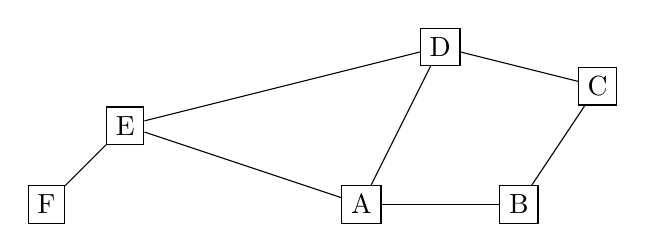
\begin{tikzpicture}
            \node[draw] (A) at (0,0) {A};
            \node[draw] (B) at (2,0) {B};
            \node[draw] (C) at (3,1.5) {C};
            \node[draw] (D) at (1,2) {D};
            \node[draw] (E) at (-3,1) {E};
            \node[draw] (F) at (-4,0) {F};
    
            \draw (B)--(A);
            \draw (A)--(E);
            \draw (D)--(E);
            \draw (A)--(D);
            \draw (D)--(C);
            \draw (C)--(B);
            \draw (F)--(E);
    
        \end{tikzpicture}
        \captionof{figure}{graphe non orienté}
        \label{oriente}
    \end{center}
\begin{aretenir}[]
    Un graphe est composé:
    \begin{itemize}
        \item de sommets ou nœuds,
        \item d'arêtes ou arcs qui relient les sommets.
    \end{itemize}
\end{aretenir}
\end{frame}

\begin{frame}
    \frametitle{}
    \begin{center}
        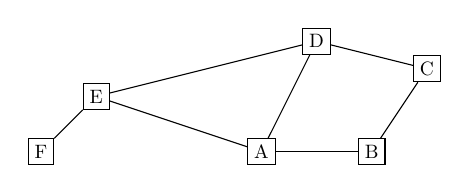
\begin{tikzpicture}[scale=0.7, transform shape]
            \node[draw] (A) at (0,0) {A};
            \node[draw] (B) at (2,0) {B};
            \node[draw] (C) at (3,1.5) {C};
            \node[draw] (D) at (1,2) {D};
            \node[draw] (E) at (-3,1) {E};
            \node[draw] (F) at (-4,0) {F};
    
            \draw (B)--(A);
            \draw (A)--(E);
            \draw (D)--(E);
            \draw (A)--(D);
            \draw (D)--(C);
            \draw (C)--(B);
            \draw (F)--(E);
    
        \end{tikzpicture}
        \captionof{figure}{graphe non orienté}
        \label{oriente}
    \end{center}
    \begin{aretenir}[]
        Pour chaque nœud on peut définir ses \textbf{prédécesseurs}.\\
        \textbf{E} est le prédécesseur de \textbf{F}.
    \end{aretenir}

\end{frame}
\subsection{Graphe pondéré}
\begin{frame}
    \frametitle{Graphe pondéré}

    \begin{center}
        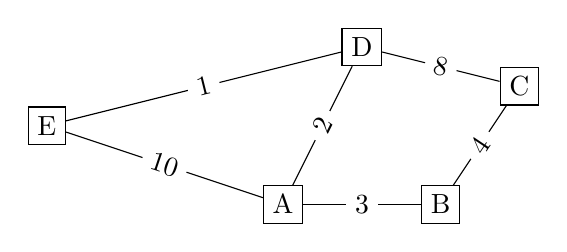
\begin{tikzpicture}
            \node[draw] (A) at (0,0) {A};
            \node[draw] (B) at (2,0) {B};
            \node[draw] (C) at (3,1.5) {C};
            \node[draw] (D) at (1,2) {D};
            \node[draw] (E) at (-3,1) {E};
    
            \draw (A)--(B) node[sloped, midway, fill=white]{3};
            \draw (A)--(E) node[sloped, midway, fill=white]{10};
            \draw (D)--(E) node[sloped, midway, fill=white]{1};
            \draw (A)--(D) node[sloped, midway, fill=white]{2};
            \draw (D)--(C) node[sloped, midway, fill=white]{8};
            \draw (C)--(B) node[sloped, midway, fill=white]{4};
    
        \end{tikzpicture}
        \captionof{figure}{graphe pondéré}
        \label{pondere}
    \end{center}
\begin{aretenir}[]
Selon le protocole mis en place la pondération pourra représenter:
\begin{itemize}
    \item RIP: le nombre de réseaux traversés,
    \item OSPF: le coût d'un réseau.
\end{itemize}
\end{aretenir}
    \note{pondération peut être négative}
\end{frame}

\section{Protocole RIP: algorithme de Bellman-Ford}
\subsection{Principe}
\begin{frame}
    \frametitle{Algorithme de Bellman-Ford: Principe}

    \begin{itemize}
        \item<1-> 1956 - 1958
        \item<2-> Richard Bellman (père programmation dynamique)
        \item<3-> Lester Ford (problème de flot maximum)
        \item<4-> redécouvert par Edward Moore en 1959
        \item<5-> Le protocole RIP applique cet algorithme.
    \end{itemize}
\note{redécouvert par Moore en 59 dans autre contexte}
\end{frame}
\begin{frame}
    \frametitle{}

    \begin{aretenir}[Remarque]
    L'algorithme de Bellman-Ford est normalement appliqué dans un graphe orienté. Cependant, si les pondérations sont toutes positives, il est possible d'utiliser un graphe non orienté.
    \end{aretenir}
    \begin{center}
        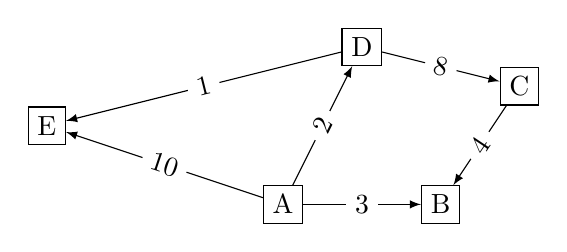
\begin{tikzpicture}
            \node[draw] (A) at (0,0) {A};
            \node[draw] (B) at (2,0) {B};
            \node[draw] (C) at (3,1.5) {C};
            \node[draw] (D) at (1,2) {D};
            \node[draw] (E) at (-3,1) {E};
    
            \draw[->,>=latex] (A)--(B) node[sloped, midway, fill=white]{3};
            \draw[->,>=latex] (A)--(E) node[sloped, midway, fill=white]{10};
            \draw[->,>=latex] (D)--(E) node[sloped, midway, fill=white]{1};
            \draw[->,>=latex] (A)--(D) node[sloped, midway, fill=white]{2};
            \draw[->,>=latex] (D)--(C) node[sloped, midway, fill=white]{8};
            \draw[->,>=latex] (C)--(B) node[sloped, midway, fill=white]{4};
    
        \end{tikzpicture}
        \captionof{figure}{graphe orienté}
        \label{pondere}
    \end{center}
\end{frame}
\begin{frame}
    \frametitle{}

    \begin{aretenir}[]
        La distance pour atteindre chaque nœud correspond à la distance pour atteindre son prédécesseur à laquelle on ajoute le poids de l'arête les séparant.
        \end{aretenir}

\end{frame}
\begin{frame}
    \frametitle{}
\note[item]{Bellman \guill{père de l'approche dynamique}}
\note[item]{\begin{aretenir}[Remarque]
    Dans le graphe figure \ref{rip} les pondérations représentent un nombre de routeurs traversés pour atteindre le nœud (routeur) suivant.
\end{aretenir}}
\begin{center}
    \begin{tikzpicture}
        \node[draw] (A) at (0,0) {A};
        \node[draw] (B) at (3,0) {B};
        \node[draw] (C) at (6,0) {C};
        \node[draw] (D) at (9,0) {D};
        \node[draw] (E) at (6,-2) {E};
        \node[draw] (F) at (6,2) {F};

        \draw (A)--(B) node[sloped, midway, fill=white]{2};
        %\draw (B)--(C) node[sloped, midway, fill=white]{6};
        \draw (C)--(D) node[sloped, midway, fill=white]{2};
        \draw (A)--(F) node[sloped, midway, fill=white]{3};
        \draw (B)--(E) node[sloped, midway, fill=white]{4};
        \draw (F)--(C) node[sloped, midway, fill=white]{2};
        \draw (E)--(C) node[sloped, midway, fill=white]{1};
        \draw (E)--(D) node[sloped, midway, fill=white]{5};
        \draw (D)--(F) node[sloped, midway, fill=white]{2};

    \end{tikzpicture}
    \captionof{figure}{graphe orienté pondéré}
    \label{rip}
\end{center}
\begin{aretenir}[]
    L'algorithme de Bellman-Ford applique une méthode récursive.
    \end{aretenir}
\end{frame}

\begin{frame}
    \frametitle{}

    \textbf{Pour chaque routeur,} on obtient un tableau contenant la distance minimale entre le routeur de départ et chaque autre routeur.
    \note{peut servir pour retrouver chemin, distance mini\dots}

\end{frame}


\subsection{Mise en application}
\begin{frame}[fragile]
    \frametitle{Mise en application}
\textbf{Initialisation:}
\begin{itemize}
    \item Créer un tableau des distances entre A et les routeurs, initialisées à l'infini.
    \item Modifier la distance vers A à 0.        
\end{itemize}
\end{frame}
\begin{frame}[fragile]
\textbf{Initialisation:}
\begin{itemize}
    \item Créer un tableau des distances entre A et les routeurs, initialisées à l'infini.
    \item Modifier la distance vers A à 0.        
\end{itemize}
\textbf{Déroulement:}
\begin{itemize}
    \item Tant que (nombre d'itérations) < (nombre de routeurs)
    \begin{itemize}
        \item Pour chaque arc du graphe
        \begin{itemize}
            \item Si (distance du routeur) > (distance de son prédécesseur + poids de l'arc entre les deux routeurs)
            \\\hspace{1cm}$\Rightarrow$ Mettre à jour distance du routeur
        \end{itemize}
    \end{itemize}
\end{itemize}
\note[item]{ligne 2 de l'algo: en effet distance de A à A = 0}
\note[item]{ligne 4: on fait autant d'itérations qu'il y a de routeurs = pire des cas $\rightarrow$ on pourra améliorer}
\end{frame}
\begin{frame}
    \frametitle{}

    \begin{aretenir}[Observations]
    \begin{itemize}
        \item On effectue autant d'itérations qu'il y a de routeurs.
        \item On regarde chaque arc à chaque tour.
    \end{itemize}
    \end{aretenir}

\end{frame}
\begin{frame}
    \frametitle{Initialisation}

    \begin{center}
        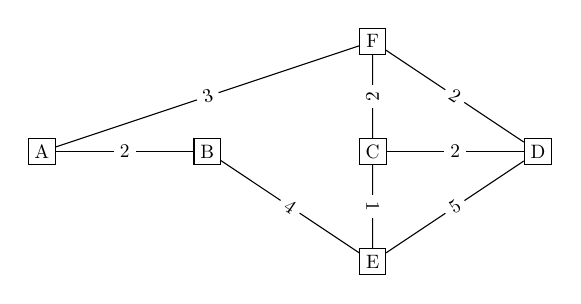
\begin{tikzpicture}[scale=0.7, transform shape]
            \node[draw] (A) at (0,0) {A};
            \node[draw] (B) at (3,0) {B};
            \node[draw] (C) at (6,0) {C};
            \node[draw] (D) at (9,0) {D};
            \node[draw] (E) at (6,-2) {E};
            \node[draw] (F) at (6,2) {F};
    
            \draw (A)--(B) node[sloped, midway, fill=white]{2};
            %\draw (B)--(C) node[sloped, midway, fill=white]{6};
            \draw (C)--(D) node[sloped, midway, fill=white]{2};
            \draw (A)--(F) node[sloped, midway, fill=white]{3};
            \draw (B)--(E) node[sloped, midway, fill=white]{4};
            \draw (F)--(C) node[sloped, midway, fill=white]{2};
            \draw (E)--(C) node[sloped, midway, fill=white]{1};
            \draw (E)--(D) node[sloped, midway, fill=white]{5};
            \draw (D)--(F) node[sloped, midway, fill=white]{2};
    
        \end{tikzpicture}
    \end{center}
    \begin{center}
        \begin{tabular}{|*{6}{c|}}
            \hline
            A & B      & C      & D      & E      & F      \\
            \hline
            0 & \infty & \infty & \infty & \infty & \infty \\
            \hline
        \end{tabular}
    \end{center}
\end{frame}

\begin{frame}
    \frametitle{Première itération}

    \begin{center}
        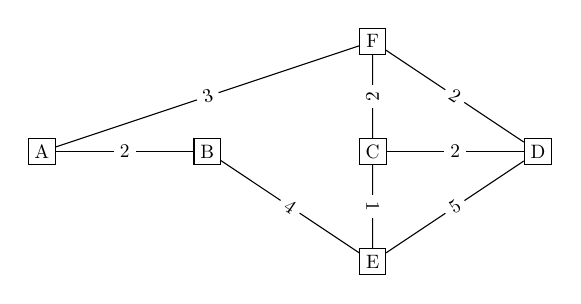
\begin{tikzpicture}[scale=0.7, transform shape]
            \node[draw] (A) at (0,0) {A};
            \node[draw] (B) at (3,0) {B};
            \node[draw] (C) at (6,0) {C};
            \node[draw] (D) at (9,0) {D};
            \node[draw] (E) at (6,-2) {E};
            \node[draw] (F) at (6,2) {F};
    
            \draw (A)--(B) node[sloped, midway, fill=white]{2};
            %\draw (B)--(C) node[sloped, midway, fill=white]{6};
            \draw (C)--(D) node[sloped, midway, fill=white]{2};
            \draw (A)--(F) node[sloped, midway, fill=white]{3};
            \draw (B)--(E) node[sloped, midway, fill=white]{4};
            \draw (F)--(C) node[sloped, midway, fill=white]{2};
            \draw (E)--(C) node[sloped, midway, fill=white]{1};
            \draw (E)--(D) node[sloped, midway, fill=white]{5};
            \draw (D)--(F) node[sloped, midway, fill=white]{2};
    
        \end{tikzpicture}
    \end{center}
    \begin{center}
        \begin{tabular}{|*{6}{c|}}
            \hline
            A & B      & C      & D      & E      & F      \\
            \hline
            0 & \textbf{2 (A)} & \infty & \infty & \infty & \infty \\
            \hline
        \end{tabular}
    \end{center}
    La distance calculée pour atteindre B correspond à la distance de son prédécesseur (A) augmentée du poids de l'arc A-B:
    $$0+2 = 2 < \infty$$
\end{frame}
\begin{frame}
    \frametitle{Première itération}

    \begin{center}
        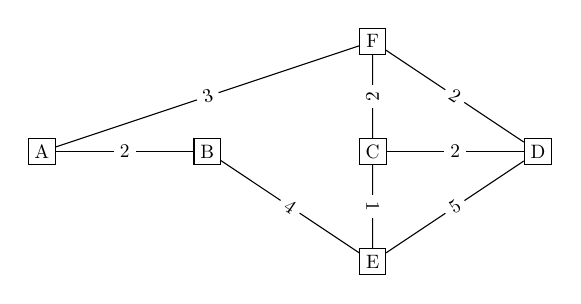
\begin{tikzpicture}[scale=0.7, transform shape]
            \node[draw] (A) at (0,0) {A};
            \node[draw] (B) at (3,0) {B};
            \node[draw] (C) at (6,0) {C};
            \node[draw] (D) at (9,0) {D};
            \node[draw] (E) at (6,-2) {E};
            \node[draw] (F) at (6,2) {F};
    
            \draw (A)--(B) node[sloped, midway, fill=white]{2};
            %\draw (B)--(C) node[sloped, midway, fill=white]{6};
            \draw (C)--(D) node[sloped, midway, fill=white]{2};
            \draw (A)--(F) node[sloped, midway, fill=white]{3};
            \draw (B)--(E) node[sloped, midway, fill=white]{4};
            \draw (F)--(C) node[sloped, midway, fill=white]{2};
            \draw (E)--(C) node[sloped, midway, fill=white]{1};
            \draw (E)--(D) node[sloped, midway, fill=white]{5};
            \draw (D)--(F) node[sloped, midway, fill=white]{2};
    
        \end{tikzpicture}
    \end{center}
    \begin{center}
        \begin{tabular}{|*{6}{c|}}
            \hline
            A & B      & C      & D      & E      & F      \\
            \hline
            0 & \textbf{2 (A)} & \infty & \infty & \infty & \infty \\
            \hline
        \end{tabular}
    \end{center}
    Second prédécesseur de B: E
    $$\infty+4 = \infty < \infty$$
\end{frame}
\begin{frame}
    \frametitle{Première itération}

    \begin{center}
        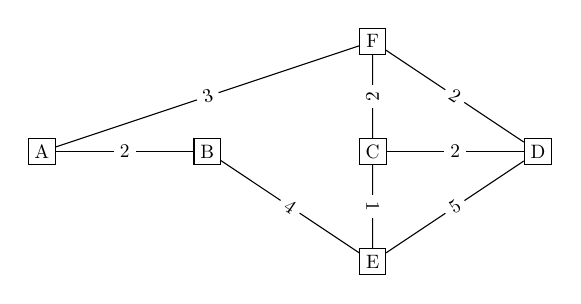
\begin{tikzpicture}[scale=0.7, transform shape]
            \node[draw] (A) at (0,0) {A};
            \node[draw] (B) at (3,0) {B};
            \node[draw] (C) at (6,0) {C};
            \node[draw] (D) at (9,0) {D};
            \node[draw] (E) at (6,-2) {E};
            \node[draw] (F) at (6,2) {F};
    
            \draw (A)--(B) node[sloped, midway, fill=white]{2};
            %\draw (B)--(C) node[sloped, midway, fill=white]{6};
            \draw (C)--(D) node[sloped, midway, fill=white]{2};
            \draw (A)--(F) node[sloped, midway, fill=white]{3};
            \draw (B)--(E) node[sloped, midway, fill=white]{4};
            \draw (F)--(C) node[sloped, midway, fill=white]{2};
            \draw (E)--(C) node[sloped, midway, fill=white]{1};
            \draw (E)--(D) node[sloped, midway, fill=white]{5};
            \draw (D)--(F) node[sloped, midway, fill=white]{2};
    
        \end{tikzpicture}
    \end{center}
    \begin{center}
        \begin{tabular}{|*{6}{c|}}
            \hline
            A & B      & C      & D      & E      & F      \\
            \hline
            0 & 2 (A) & \infty & \infty & \infty & \infty \\
            \hline
        \end{tabular}
    \end{center}
    Premier prédécesseur de C: D
    $$\infty+1 = \infty \nless \infty$$
    \note{On est toujours dans la première itération; on vérifie chaque arc.}
\end{frame}

\begin{frame}
    \frametitle{Première itération}

    \begin{center}
        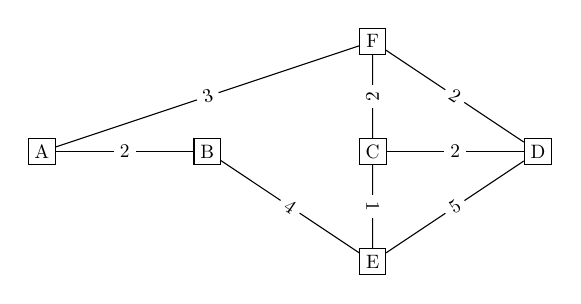
\begin{tikzpicture}[scale=0.7, transform shape]
            \node[draw] (A) at (0,0) {A};
            \node[draw] (B) at (3,0) {B};
            \node[draw] (C) at (6,0) {C};
            \node[draw] (D) at (9,0) {D};
            \node[draw] (E) at (6,-2) {E};
            \node[draw] (F) at (6,2) {F};
    
            \draw (A)--(B) node[sloped, midway, fill=white]{2};
            %\draw (B)--(C) node[sloped, midway, fill=white]{6};
            \draw (C)--(D) node[sloped, midway, fill=white]{2};
            \draw (A)--(F) node[sloped, midway, fill=white]{3};
            \draw (B)--(E) node[sloped, midway, fill=white]{4};
            \draw (F)--(C) node[sloped, midway, fill=white]{2};
            \draw (E)--(C) node[sloped, midway, fill=white]{1};
            \draw (E)--(D) node[sloped, midway, fill=white]{5};
            \draw (D)--(F) node[sloped, midway, fill=white]{2};
    
        \end{tikzpicture}
    \end{center}
    \begin{center}
        \begin{tabular}{|*{6}{c|}}
            \hline
            A & B      & C      & D      & E      & F      \\
            \hline
            0 & 2 (A) & \infty & \infty & \infty & \infty \\
            \hline
        \end{tabular}
    \end{center}
    Deuxième prédécesseur de C: E
    $$\infty+1 = \infty \nless \infty$$
\end{frame}
\begin{frame}
    \frametitle{Première itération}

    \begin{center}
        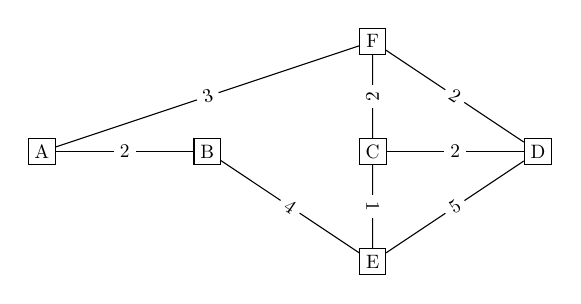
\begin{tikzpicture}[scale=0.7, transform shape]
            \node[draw] (A) at (0,0) {A};
            \node[draw] (B) at (3,0) {B};
            \node[draw] (C) at (6,0) {C};
            \node[draw] (D) at (9,0) {D};
            \node[draw] (E) at (6,-2) {E};
            \node[draw] (F) at (6,2) {F};
    
            \draw (A)--(B) node[sloped, midway, fill=white]{2};
            %\draw (B)--(C) node[sloped, midway, fill=white]{6};
            \draw (C)--(D) node[sloped, midway, fill=white]{2};
            \draw (A)--(F) node[sloped, midway, fill=white]{3};
            \draw (B)--(E) node[sloped, midway, fill=white]{4};
            \draw (F)--(C) node[sloped, midway, fill=white]{2};
            \draw (E)--(C) node[sloped, midway, fill=white]{1};
            \draw (E)--(D) node[sloped, midway, fill=white]{5};
            \draw (D)--(F) node[sloped, midway, fill=white]{2};
    
        \end{tikzpicture}
    \end{center}
    \begin{center}
        \begin{tabular}{|*{6}{c|}}
            \hline
            A & B      & C      & D      & E      & F      \\
            \hline
            0 & 2 (A) & \infty & \infty & \infty & \infty \\
            \hline
        \end{tabular}
    \end{center}
    Troisième prédécesseur de C: F
    $$\infty+2 = \infty \nless  \infty$$
\end{frame}
\begin{frame}
    \frametitle{}

    \begin{activite}
        Continuer de dérouler la première itération de l'algorithme sur le graphe.
    \end{activite}
    \begin{center}
        \begin{tikzpicture}[scale=0.9, transform shape]
            \node[draw] (A) at (0,0) {A};
            \node[draw] (B) at (3,0) {B};
            \node[draw] (C) at (6,0) {C};
            \node[draw] (D) at (9,0) {D};
            \node[draw] (E) at (6,-2) {E};
            \node[draw] (F) at (6,2) {F};
    
            \draw (A)--(B) node[sloped, midway, fill=white]{2};
            %\draw (B)--(C) node[sloped, midway, fill=white]{6};
            \draw (C)--(D) node[sloped, midway, fill=white]{2};
            \draw (A)--(F) node[sloped, midway, fill=white]{3};
            \draw (B)--(E) node[sloped, midway, fill=white]{4};
            \draw (F)--(C) node[sloped, midway, fill=white]{2};
            \draw (E)--(C) node[sloped, midway, fill=white]{1};
            \draw (E)--(D) node[sloped, midway, fill=white]{5};
            \draw (D)--(F) node[sloped, midway, fill=white]{2};
    
        \end{tikzpicture}
    \end{center}
\end{frame}
\begin{frame}
    \frametitle{Première itération}

    \begin{center}
        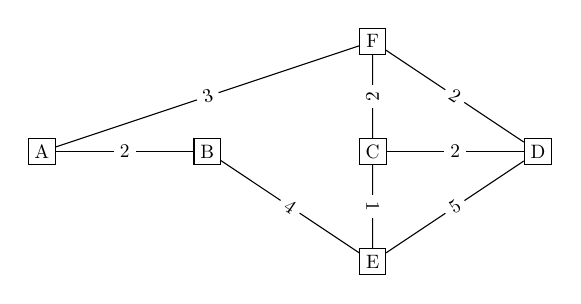
\begin{tikzpicture}[scale=0.7, transform shape]
            \node[draw] (A) at (0,0) {A};
            \node[draw] (B) at (3,0) {B};
            \node[draw] (C) at (6,0) {C};
            \node[draw] (D) at (9,0) {D};
            \node[draw] (E) at (6,-2) {E};
            \node[draw] (F) at (6,2) {F};
    
            \draw (A)--(B) node[sloped, midway, fill=white]{2};
            %\draw (B)--(C) node[sloped, midway, fill=white]{6};
            \draw (C)--(D) node[sloped, midway, fill=white]{2};
            \draw (A)--(F) node[sloped, midway, fill=white]{3};
            \draw (B)--(E) node[sloped, midway, fill=white]{4};
            \draw (F)--(C) node[sloped, midway, fill=white]{2};
            \draw (E)--(C) node[sloped, midway, fill=white]{1};
            \draw (E)--(D) node[sloped, midway, fill=white]{5};
            \draw (D)--(F) node[sloped, midway, fill=white]{2};
    
        \end{tikzpicture}
    \end{center}
    \begin{center}
        \begin{tabular}{|*{6}{c|}}
            \hline
            A & B      & C      & D      & E      & F      \\
            \hline
            0 & 2 (A) & \infty & \infty & \infty & \infty \\
            \hline
        \end{tabular}
    \end{center}
    Même constat pour D
\end{frame}

\begin{frame}
    \frametitle{Première itération}

    \begin{center}
        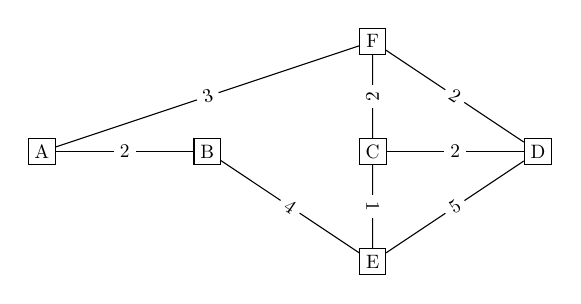
\begin{tikzpicture}[scale=0.7, transform shape]
            \node[draw] (A) at (0,0) {A};
            \node[draw] (B) at (3,0) {B};
            \node[draw] (C) at (6,0) {C};
            \node[draw] (D) at (9,0) {D};
            \node[draw] (E) at (6,-2) {E};
            \node[draw] (F) at (6,2) {F};
    
            \draw (A)--(B) node[sloped, midway, fill=white]{2};
            %\draw (B)--(C) node[sloped, midway, fill=white]{6};
            \draw (C)--(D) node[sloped, midway, fill=white]{2};
            \draw (A)--(F) node[sloped, midway, fill=white]{3};
            \draw (B)--(E) node[sloped, midway, fill=white]{4};
            \draw (F)--(C) node[sloped, midway, fill=white]{2};
            \draw (E)--(C) node[sloped, midway, fill=white]{1};
            \draw (E)--(D) node[sloped, midway, fill=white]{5};
            \draw (D)--(F) node[sloped, midway, fill=white]{2};
    
        \end{tikzpicture}
    \end{center}
    \begin{center}
        \begin{tabular}{|*{6}{c|}}
            \hline
            A & B      & C      & D      & E      & F      \\
            \hline
            0 & 2 (A) & \infty & \infty & \textbf{6 (B)} & \infty \\
            \hline
        \end{tabular}
    \end{center}
    Premier prédécesseur de E: B
    $$2+4 = 6 <  \infty$$
\end{frame}
\begin{frame}
    \frametitle{Première itération}

    \begin{center}
        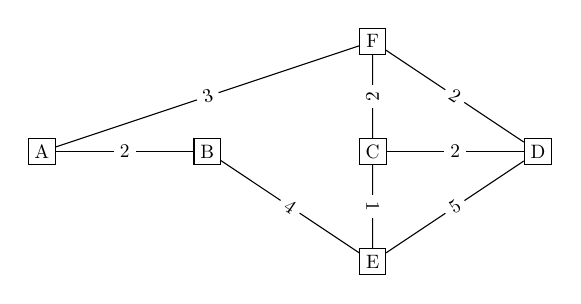
\begin{tikzpicture}[scale=0.7, transform shape]
            \node[draw] (A) at (0,0) {A};
            \node[draw] (B) at (3,0) {B};
            \node[draw] (C) at (6,0) {C};
            \node[draw] (D) at (9,0) {D};
            \node[draw] (E) at (6,-2) {E};
            \node[draw] (F) at (6,2) {F};
    
            \draw (A)--(B) node[sloped, midway, fill=white]{2};
            %\draw (B)--(C) node[sloped, midway, fill=white]{6};
            \draw (C)--(D) node[sloped, midway, fill=white]{2};
            \draw (A)--(F) node[sloped, midway, fill=white]{3};
            \draw (B)--(E) node[sloped, midway, fill=white]{4};
            \draw (F)--(C) node[sloped, midway, fill=white]{2};
            \draw (E)--(C) node[sloped, midway, fill=white]{1};
            \draw (E)--(D) node[sloped, midway, fill=white]{5};
            \draw (D)--(F) node[sloped, midway, fill=white]{2};
    
        \end{tikzpicture}
    \end{center}
    \begin{center}
        \begin{tabular}{|*{6}{c|}}
            \hline
            A & B      & C      & D      & E      & F      \\
            \hline
            0 & 2 (A) & \infty & \infty & \textbf{6 (B)} & \infty \\
            \hline
        \end{tabular}
    \end{center}
    Deuxième prédécesseur de E: C
    $$\infty+1 = \infty >  6$$
\end{frame}
\begin{frame}
    \frametitle{Première itération}

    \begin{center}
        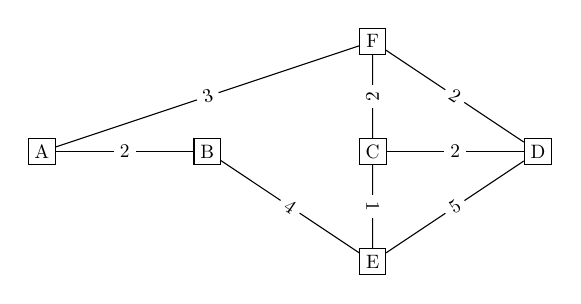
\begin{tikzpicture}[scale=0.7, transform shape]
            \node[draw] (A) at (0,0) {A};
            \node[draw] (B) at (3,0) {B};
            \node[draw] (C) at (6,0) {C};
            \node[draw] (D) at (9,0) {D};
            \node[draw] (E) at (6,-2) {E};
            \node[draw] (F) at (6,2) {F};
    
            \draw (A)--(B) node[sloped, midway, fill=white]{2};
            %\draw (B)--(C) node[sloped, midway, fill=white]{6};
            \draw (C)--(D) node[sloped, midway, fill=white]{2};
            \draw (A)--(F) node[sloped, midway, fill=white]{3};
            \draw (B)--(E) node[sloped, midway, fill=white]{4};
            \draw (F)--(C) node[sloped, midway, fill=white]{2};
            \draw (E)--(C) node[sloped, midway, fill=white]{1};
            \draw (E)--(D) node[sloped, midway, fill=white]{5};
            \draw (D)--(F) node[sloped, midway, fill=white]{2};
    
        \end{tikzpicture}
    \end{center}
    \begin{center}
        \begin{tabular}{|*{6}{c|}}
            \hline
            A & B      & C      & D      & E      & F      \\
            \hline
            0 & 2 (A) & \infty & \infty & \textbf{6 (B)} & \infty \\
            \hline
        \end{tabular}
    \end{center}
    Troisième prédécesseur de E: D
    $$\infty+5 = \infty >  6$$
\end{frame}
\begin{frame}
    \frametitle{Première itération}

    \begin{center}
        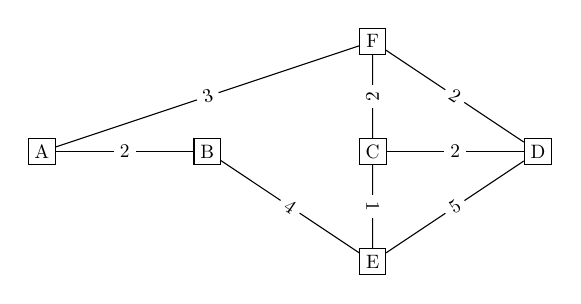
\begin{tikzpicture}[scale=0.7, transform shape]
            \node[draw] (A) at (0,0) {A};
            \node[draw] (B) at (3,0) {B};
            \node[draw] (C) at (6,0) {C};
            \node[draw] (D) at (9,0) {D};
            \node[draw] (E) at (6,-2) {E};
            \node[draw] (F) at (6,2) {F};
    
            \draw (A)--(B) node[sloped, midway, fill=white]{2};
            %\draw (B)--(C) node[sloped, midway, fill=white]{6};
            \draw (C)--(D) node[sloped, midway, fill=white]{2};
            \draw (A)--(F) node[sloped, midway, fill=white]{3};
            \draw (B)--(E) node[sloped, midway, fill=white]{4};
            \draw (F)--(C) node[sloped, midway, fill=white]{2};
            \draw (E)--(C) node[sloped, midway, fill=white]{1};
            \draw (E)--(D) node[sloped, midway, fill=white]{5};
            \draw (D)--(F) node[sloped, midway, fill=white]{2};
    
        \end{tikzpicture}
    \end{center}
    \begin{center}
        \begin{tabular}{|*{6}{c|}}
            \hline
            A & B      & C      & D      & E      & F      \\
            \hline
            0 & 2 (A)& \infty & \infty & 6 (B) & \textbf{3 (A)}  \\
            \hline
        \end{tabular}
    \end{center}
    Premier prédécesseur de F: A
    $$0+3 = 3 <  \infty$$
\end{frame}

\begin{frame}
    \frametitle{Première itération}

    \begin{center}
        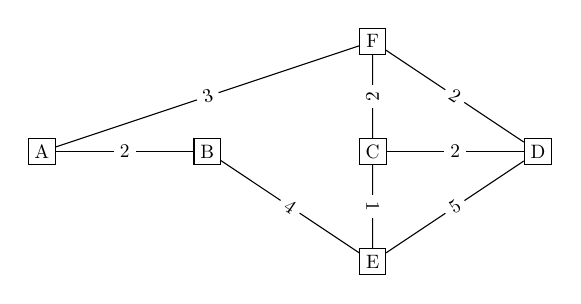
\begin{tikzpicture}[scale=0.7, transform shape]
            \node[draw] (A) at (0,0) {A};
            \node[draw] (B) at (3,0) {B};
            \node[draw] (C) at (6,0) {C};
            \node[draw] (D) at (9,0) {D};
            \node[draw] (E) at (6,-2) {E};
            \node[draw] (F) at (6,2) {F};
    
            \draw (A)--(B) node[sloped, midway, fill=white]{2};
            %\draw (B)--(C) node[sloped, midway, fill=white]{6};
            \draw (C)--(D) node[sloped, midway, fill=white]{2};
            \draw (A)--(F) node[sloped, midway, fill=white]{3};
            \draw (B)--(E) node[sloped, midway, fill=white]{4};
            \draw (F)--(C) node[sloped, midway, fill=white]{2};
            \draw (E)--(C) node[sloped, midway, fill=white]{1};
            \draw (E)--(D) node[sloped, midway, fill=white]{5};
            \draw (D)--(F) node[sloped, midway, fill=white]{2};
    
        \end{tikzpicture}
    \end{center}
    \begin{center}
        \begin{tabular}{|*{6}{c|}}
            \hline
            A & B      & C      & D      & E      & F      \\
            \hline
            0 & 2 (A)& \infty & \infty & 6 (B) & 3 (A) \\
            \hline
        \end{tabular}
    \end{center}
    Deuxième prédécesseur de F: C
    $$\infty+2 = \infty \nless  3$$
\end{frame}
\begin{frame}
    \frametitle{Première itération}

    \begin{center}
        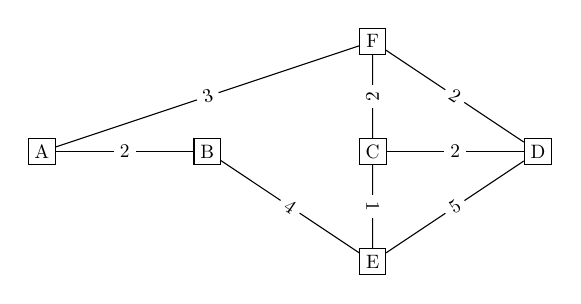
\begin{tikzpicture}[scale=0.7, transform shape]
            \node[draw] (A) at (0,0) {A};
            \node[draw] (B) at (3,0) {B};
            \node[draw] (C) at (6,0) {C};
            \node[draw] (D) at (9,0) {D};
            \node[draw] (E) at (6,-2) {E};
            \node[draw] (F) at (6,2) {F};
    
            \draw (A)--(B) node[sloped, midway, fill=white]{2};
            %\draw (B)--(C) node[sloped, midway, fill=white]{6};
            \draw (C)--(D) node[sloped, midway, fill=white]{2};
            \draw (A)--(F) node[sloped, midway, fill=white]{3};
            \draw (B)--(E) node[sloped, midway, fill=white]{4};
            \draw (F)--(C) node[sloped, midway, fill=white]{2};
            \draw (E)--(C) node[sloped, midway, fill=white]{1};
            \draw (E)--(D) node[sloped, midway, fill=white]{5};
            \draw (D)--(F) node[sloped, midway, fill=white]{2};
    
        \end{tikzpicture}
    \end{center}
    \begin{center}
        \begin{tabular}{|*{6}{c|}}
            \hline
            A & B      & C      & D      & E      & F      \\
            \hline
            0 & 2 (A)& \infty & \infty & 6 (B) & 3 (A) \\
            \hline
        \end{tabular}
    \end{center}
    Troisième prédécesseur de F: D
    $$\infty+2 = \infty \nless  3$$
\end{frame}
\begin{frame}
    \frametitle{Première itération}

    \begin{center}
        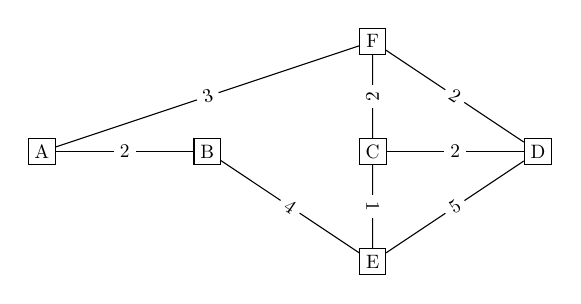
\begin{tikzpicture}[scale=0.7, transform shape]
            \node[draw] (A) at (0,0) {A};
            \node[draw] (B) at (3,0) {B};
            \node[draw] (C) at (6,0) {C};
            \node[draw] (D) at (9,0) {D};
            \node[draw] (E) at (6,-2) {E};
            \node[draw] (F) at (6,2) {F};
    
            \draw (A)--(B) node[sloped, midway, fill=white]{2};
            %\draw (B)--(C) node[sloped, midway, fill=white]{6};
            \draw (C)--(D) node[sloped, midway, fill=white]{2};
            \draw (A)--(F) node[sloped, midway, fill=white]{3};
            \draw (B)--(E) node[sloped, midway, fill=white]{4};
            \draw (F)--(C) node[sloped, midway, fill=white]{2};
            \draw (E)--(C) node[sloped, midway, fill=white]{1};
            \draw (E)--(D) node[sloped, midway, fill=white]{5};
            \draw (D)--(F) node[sloped, midway, fill=white]{2};
    
        \end{tikzpicture}
    \end{center}
    \begin{center}
        \begin{tabular}{|*{6}{c|}}
            \hline
            A & B      & C      & D      & E      & F      \\
            \hline
            0 & 2 (A) & \infty & \infty & 6 (B) & 3 (A) \\
            \hline
        \end{tabular}
    \end{center}
    \begin{center}
        {\LARGE Fin de la première itération}
    \end{center}
\end{frame}

\begin{frame}
    \frametitle{Deuxième itération}

    \begin{center}
        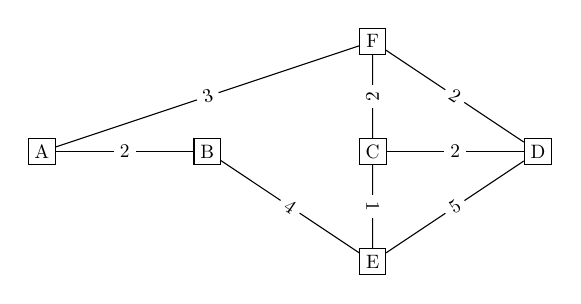
\begin{tikzpicture}[scale=0.7, transform shape]
            \node[draw] (A) at (0,0) {A};
            \node[draw] (B) at (3,0) {B};
            \node[draw] (C) at (6,0) {C};
            \node[draw] (D) at (9,0) {D};
            \node[draw] (E) at (6,-2) {E};
            \node[draw] (F) at (6,2) {F};
    
            \draw (A)--(B) node[sloped, midway, fill=white]{2};
            %\draw (B)--(C) node[sloped, midway, fill=white]{6};
            \draw (C)--(D) node[sloped, midway, fill=white]{2};
            \draw (A)--(F) node[sloped, midway, fill=white]{3};
            \draw (B)--(E) node[sloped, midway, fill=white]{4};
            \draw (F)--(C) node[sloped, midway, fill=white]{2};
            \draw (E)--(C) node[sloped, midway, fill=white]{1};
            \draw (E)--(D) node[sloped, midway, fill=white]{5};
            \draw (D)--(F) node[sloped, midway, fill=white]{2};
    
        \end{tikzpicture}
    \end{center}
    \begin{center}
        \begin{tabular}{|*{6}{c|}}
            \hline
            A & B      & C      & D      & E      & F      \\
            \hline
            0 & 2 (A) & \infty & \infty & 6 (B) & 3 (A) \\
            \hline
            0 & 2 (A) & \infty & \infty & 6 (B) & 3 (A) \\
            \hline
        \end{tabular}
    \end{center}
    {\Large Pas de modification pour A et B}
\end{frame}
\begin{frame}
    \frametitle{Deuxième itération}

    \begin{center}
        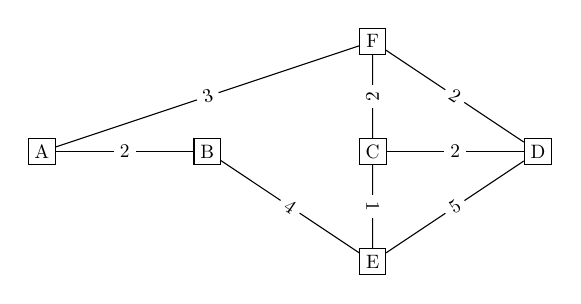
\begin{tikzpicture}[scale=0.7, transform shape]
            \node[draw] (A) at (0,0) {A};
            \node[draw] (B) at (3,0) {B};
            \node[draw] (C) at (6,0) {C};
            \node[draw] (D) at (9,0) {D};
            \node[draw] (E) at (6,-2) {E};
            \node[draw] (F) at (6,2) {F};
    
            \draw (A)--(B) node[sloped, midway, fill=white]{2};
            %\draw (B)--(C) node[sloped, midway, fill=white]{6};
            \draw (C)--(D) node[sloped, midway, fill=white]{2};
            \draw (A)--(F) node[sloped, midway, fill=white]{3};
            \draw (B)--(E) node[sloped, midway, fill=white]{4};
            \draw (F)--(C) node[sloped, midway, fill=white]{2};
            \draw (E)--(C) node[sloped, midway, fill=white]{1};
            \draw (E)--(D) node[sloped, midway, fill=white]{5};
            \draw (D)--(F) node[sloped, midway, fill=white]{2};
    
        \end{tikzpicture}
    \end{center}
    \begin{center}
        \begin{tabular}{|*{6}{c|}}
            \hline
            A & B      & C      & D      & E      & F      \\
            \hline
            0 & 2 (A) & \infty & \infty & 6 (B) & 3 (A) \\
            \hline
            0 & 2 (A) & \textbf{7 (E)} & \infty & 6 (B)& 3 (A)\\
            \hline
        \end{tabular}
    \end{center}
    Premier prédécesseur de C: D
    $$\infty+2 = \infty \nless \infty$$
    
\end{frame}
\begin{frame}
    \frametitle{Deuxième itération}

    \begin{center}
        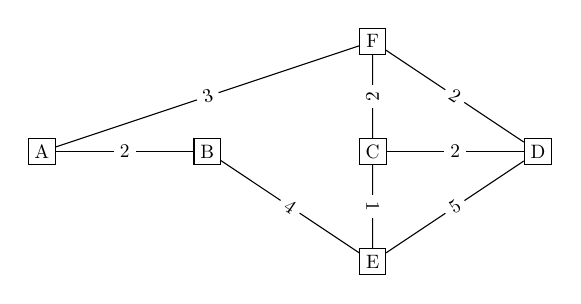
\begin{tikzpicture}[scale=0.7, transform shape]
            \node[draw] (A) at (0,0) {A};
            \node[draw] (B) at (3,0) {B};
            \node[draw] (C) at (6,0) {C};
            \node[draw] (D) at (9,0) {D};
            \node[draw] (E) at (6,-2) {E};
            \node[draw] (F) at (6,2) {F};
    
            \draw (A)--(B) node[sloped, midway, fill=white]{2};
            %\draw (B)--(C) node[sloped, midway, fill=white]{6};
            \draw (C)--(D) node[sloped, midway, fill=white]{2};
            \draw (A)--(F) node[sloped, midway, fill=white]{3};
            \draw (B)--(E) node[sloped, midway, fill=white]{4};
            \draw (F)--(C) node[sloped, midway, fill=white]{2};
            \draw (E)--(C) node[sloped, midway, fill=white]{1};
            \draw (E)--(D) node[sloped, midway, fill=white]{5};
            \draw (D)--(F) node[sloped, midway, fill=white]{2};
    
        \end{tikzpicture}
    \end{center}
    \begin{center}
        \begin{tabular}{|*{6}{c|}}
            \hline
            A & B      & C      & D      & E      & F      \\
            \hline
            0 & 2 (A) & \infty & \infty & 6 (B) & 3 (A) \\
            \hline
            0 & 2 (A) & \textbf{7 (E)} & \infty & 6 (B)& 3 (A)\\
            \hline
        \end{tabular}
    \end{center}
    Deuxième prédécesseur de C: E
    $$6+1 = 7 < \infty$$
    
\end{frame}

\begin{frame}
    \frametitle{Deuxième itération}

    \begin{center}
        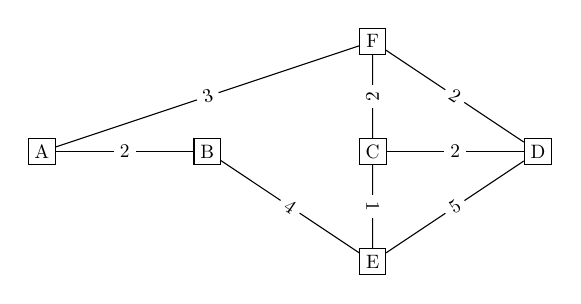
\begin{tikzpicture}[scale=0.7, transform shape]
            \node[draw] (A) at (0,0) {A};
            \node[draw] (B) at (3,0) {B};
            \node[draw] (C) at (6,0) {C};
            \node[draw] (D) at (9,0) {D};
            \node[draw] (E) at (6,-2) {E};
            \node[draw] (F) at (6,2) {F};
    
            \draw (A)--(B) node[sloped, midway, fill=white]{2};
            %\draw (B)--(C) node[sloped, midway, fill=white]{6};
            \draw (C)--(D) node[sloped, midway, fill=white]{2};
            \draw (A)--(F) node[sloped, midway, fill=white]{3};
            \draw (B)--(E) node[sloped, midway, fill=white]{4};
            \draw (F)--(C) node[sloped, midway, fill=white]{2};
            \draw (E)--(C) node[sloped, midway, fill=white]{1};
            \draw (E)--(D) node[sloped, midway, fill=white]{5};
            \draw (D)--(F) node[sloped, midway, fill=white]{2};
    
        \end{tikzpicture}
    \end{center}
    \begin{center}
        \begin{tabular}{|*{6}{c|}}
            \hline
            A & B      & C      & D      & E      & F      \\
            \hline
            0 & 2 (A) & \infty & \infty & 6 (B) & 3 (A) \\
            \hline
            0 & 2 (A) & \textbf{5 (F)} & \infty & 6 (B) & 3 (A) \\
            \hline
        \end{tabular}
    \end{center}
    Troisième prédécesseur de C: F
    $$3+2 = 5 < 7$$
    
\end{frame}

\begin{frame}
    \frametitle{Deuxième itération}

    \begin{center}
        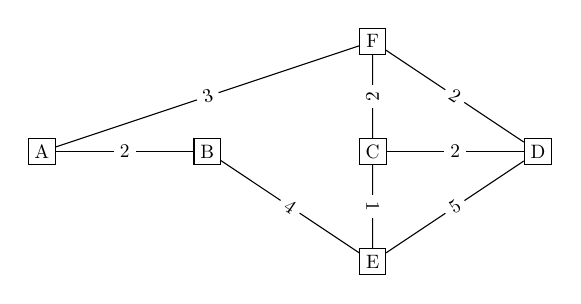
\begin{tikzpicture}[scale=0.7, transform shape]
            \node[draw] (A) at (0,0) {A};
            \node[draw] (B) at (3,0) {B};
            \node[draw] (C) at (6,0) {C};
            \node[draw] (D) at (9,0) {D};
            \node[draw] (E) at (6,-2) {E};
            \node[draw] (F) at (6,2) {F};
    
            \draw (A)--(B) node[sloped, midway, fill=white]{2};
            %\draw (B)--(C) node[sloped, midway, fill=white]{6};
            \draw (C)--(D) node[sloped, midway, fill=white]{2};
            \draw (A)--(F) node[sloped, midway, fill=white]{3};
            \draw (B)--(E) node[sloped, midway, fill=white]{4};
            \draw (F)--(C) node[sloped, midway, fill=white]{2};
            \draw (E)--(C) node[sloped, midway, fill=white]{1};
            \draw (E)--(D) node[sloped, midway, fill=white]{5};
            \draw (D)--(F) node[sloped, midway, fill=white]{2};
    
        \end{tikzpicture}
    \end{center}
    \begin{center}
        \begin{tabular}{|*{6}{c|}}
            \hline
            A & B      & C      & D      & E      & F      \\
            \hline
            0 & 2 (A) & \infty & \infty & 6 (B) & 3 (A) \\
            \hline
            0 & 2 (A) & 5 (F) & \textbf{7 (C)} & 6 (B) & 3 (A) \\
            \hline
        \end{tabular}
    \end{center}
    Premier prédécesseur de D: C
    $$5+2 = 7 < \infty$$
    
\end{frame}

\begin{frame}
    \frametitle{Deuxième itération}

    \begin{center}
        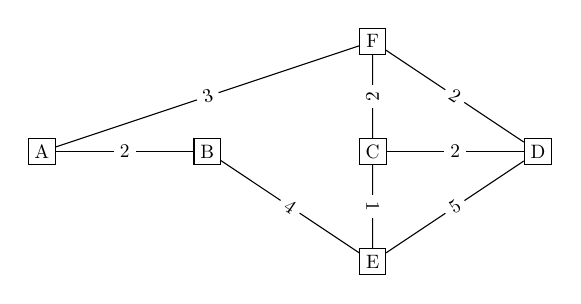
\begin{tikzpicture}[scale=0.7, transform shape]
            \node[draw] (A) at (0,0) {A};
            \node[draw] (B) at (3,0) {B};
            \node[draw] (C) at (6,0) {C};
            \node[draw] (D) at (9,0) {D};
            \node[draw] (E) at (6,-2) {E};
            \node[draw] (F) at (6,2) {F};
    
            \draw (A)--(B) node[sloped, midway, fill=white]{2};
            %\draw (B)--(C) node[sloped, midway, fill=white]{6};
            \draw (C)--(D) node[sloped, midway, fill=white]{2};
            \draw (A)--(F) node[sloped, midway, fill=white]{3};
            \draw (B)--(E) node[sloped, midway, fill=white]{4};
            \draw (F)--(C) node[sloped, midway, fill=white]{2};
            \draw (E)--(C) node[sloped, midway, fill=white]{1};
            \draw (E)--(D) node[sloped, midway, fill=white]{5};
            \draw (D)--(F) node[sloped, midway, fill=white]{2};
    
        \end{tikzpicture}
    \end{center}
    \begin{center}
        \begin{tabular}{|*{6}{c|}}
            \hline
            A & B      & C      & D      & E      & F      \\
            \hline
            0 & 2 (A) & \infty & \infty & 6 (B) & 3 (A) \\
            \hline
            0 & 2 (A) & 5 (F) & 7 (C) & 6 (B) & 3 (A) \\
            \hline
        \end{tabular}
    \end{center}
    Second prédécesseur de D: E
    $$6+5 = 11 \nless 7$$
    
\end{frame}
\begin{frame}
    \frametitle{Deuxième itération}

    \begin{center}
        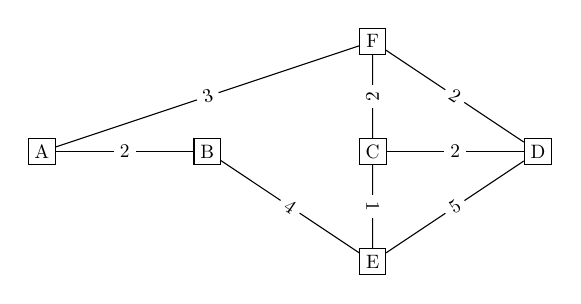
\begin{tikzpicture}[scale=0.7, transform shape]
            \node[draw] (A) at (0,0) {A};
            \node[draw] (B) at (3,0) {B};
            \node[draw] (C) at (6,0) {C};
            \node[draw] (D) at (9,0) {D};
            \node[draw] (E) at (6,-2) {E};
            \node[draw] (F) at (6,2) {F};
    
            \draw (A)--(B) node[sloped, midway, fill=white]{2};
            %\draw (B)--(C) node[sloped, midway, fill=white]{6};
            \draw (C)--(D) node[sloped, midway, fill=white]{2};
            \draw (A)--(F) node[sloped, midway, fill=white]{3};
            \draw (B)--(E) node[sloped, midway, fill=white]{4};
            \draw (F)--(C) node[sloped, midway, fill=white]{2};
            \draw (E)--(C) node[sloped, midway, fill=white]{1};
            \draw (E)--(D) node[sloped, midway, fill=white]{5};
            \draw (D)--(F) node[sloped, midway, fill=white]{2};
    
        \end{tikzpicture}
    \end{center}
    \begin{center}
        \begin{tabular}{|*{6}{c|}}
            \hline
            A & B      & C      & D      & E      & F      \\
            \hline
            0 & 2 (A) & \infty & \infty & 6 (B) & 3 (A) \\
            \hline
            0 & 2 (A) & 5 (F) & \textbf{5 (F)} & 6 (B) & 3 (A) \\
            \hline
        \end{tabular}
    \end{center}
    Troisième prédécesseur de D: F
    $$3+2 = 5 < 7$$
    
\end{frame}
\begin{frame}
    \frametitle{Deuxième itération}

    \begin{center}
        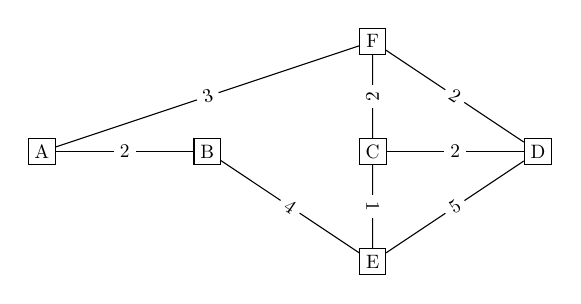
\begin{tikzpicture}[scale=0.7, transform shape]
            \node[draw] (A) at (0,0) {A};
            \node[draw] (B) at (3,0) {B};
            \node[draw] (C) at (6,0) {C};
            \node[draw] (D) at (9,0) {D};
            \node[draw] (E) at (6,-2) {E};
            \node[draw] (F) at (6,2) {F};
    
            \draw (A)--(B) node[sloped, midway, fill=white]{2};
            %\draw (B)--(C) node[sloped, midway, fill=white]{6};
            \draw (C)--(D) node[sloped, midway, fill=white]{2};
            \draw (A)--(F) node[sloped, midway, fill=white]{3};
            \draw (B)--(E) node[sloped, midway, fill=white]{4};
            \draw (F)--(C) node[sloped, midway, fill=white]{2};
            \draw (E)--(C) node[sloped, midway, fill=white]{1};
            \draw (E)--(D) node[sloped, midway, fill=white]{5};
            \draw (D)--(F) node[sloped, midway, fill=white]{2};
    
        \end{tikzpicture}
    \end{center}
    \begin{center}
        \begin{tabular}{|*{6}{c|}}
            \hline
            A & B      & C      & D      & E      & F      \\
            \hline
            0 & 2 (A) & \infty & \infty & 6 (B) & 3 (A) \\
            \hline
            0 & 2 (A) & 5 (F) & 5 (F) & 6 (B) & 3 (A) \\
            \hline
        \end{tabular}
    \end{center}
    \begin{center}
        {\LARGE Pas de changement pour E et F}
    \end{center}
    
\end{frame}
\begin{frame}
    \frametitle{Deuxième itération}

    \begin{center}
        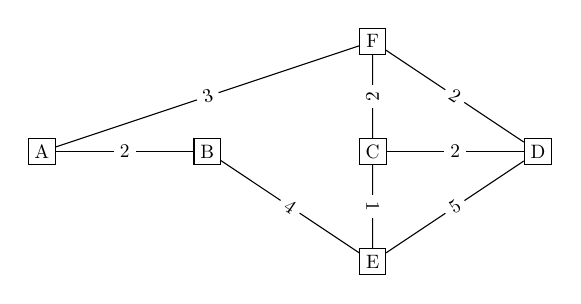
\begin{tikzpicture}[scale=0.7, transform shape]
            \node[draw] (A) at (0,0) {A};
            \node[draw] (B) at (3,0) {B};
            \node[draw] (C) at (6,0) {C};
            \node[draw] (D) at (9,0) {D};
            \node[draw] (E) at (6,-2) {E};
            \node[draw] (F) at (6,2) {F};
    
            \draw (A)--(B) node[sloped, midway, fill=white]{2};
            %\draw (B)--(C) node[sloped, midway, fill=white]{6};
            \draw (C)--(D) node[sloped, midway, fill=white]{2};
            \draw (A)--(F) node[sloped, midway, fill=white]{3};
            \draw (B)--(E) node[sloped, midway, fill=white]{4};
            \draw (F)--(C) node[sloped, midway, fill=white]{2};
            \draw (E)--(C) node[sloped, midway, fill=white]{1};
            \draw (E)--(D) node[sloped, midway, fill=white]{5};
            \draw (D)--(F) node[sloped, midway, fill=white]{2};
    
        \end{tikzpicture}
    \end{center}
    \begin{center}
        \begin{tabular}{|*{6}{c|}}
            \hline
            A & B      & C      & D      & E      & F      \\
            \hline
            0 & 2 (A) & \infty & \infty & 6 (B) & 3 (A) \\
            \hline
            0 & 2 (A) & 5 (F) & 5 (F) & 6 (B) & 3 (A) \\
            \hline
        \end{tabular}
    \end{center}
    \begin{center}
        {\LARGE Fin de la deuxième itération}
    \end{center}
    
\end{frame}

\begin{frame}
    \frametitle{Troisième itération}

    \begin{center}
        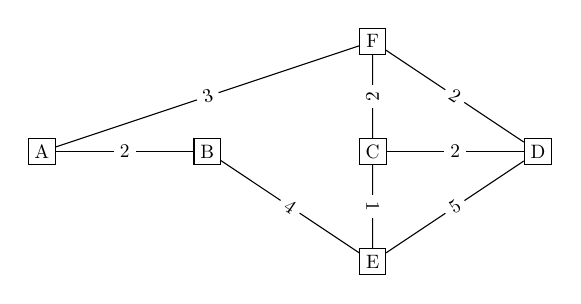
\begin{tikzpicture}[scale=0.7, transform shape]
            \node[draw] (A) at (0,0) {A};
            \node[draw] (B) at (3,0) {B};
            \node[draw] (C) at (6,0) {C};
            \node[draw] (D) at (9,0) {D};
            \node[draw] (E) at (6,-2) {E};
            \node[draw] (F) at (6,2) {F};
    
            \draw (A)--(B) node[sloped, midway, fill=white]{2};
            %\draw (B)--(C) node[sloped, midway, fill=white]{6};
            \draw (C)--(D) node[sloped, midway, fill=white]{2};
            \draw (A)--(F) node[sloped, midway, fill=white]{3};
            \draw (B)--(E) node[sloped, midway, fill=white]{4};
            \draw (F)--(C) node[sloped, midway, fill=white]{2};
            \draw (E)--(C) node[sloped, midway, fill=white]{1};
            \draw (E)--(D) node[sloped, midway, fill=white]{5};
            \draw (D)--(F) node[sloped, midway, fill=white]{2};
    
        \end{tikzpicture}
    \end{center}
    \begin{center}
        \begin{tabular}{|*{6}{c|}}
            \hline
            A & B      & C      & D      & E      & F      \\
            \hline
            0 & 2 (A) & \infty & \infty & 6 (B) & 3 (A) \\
            \hline
            0 & 2 (A) & 5 (F) & 5 (F) & 6 (B) & 3 (A) \\
            \hline
            0 & 2 (A) & 5 (F) & 5 (F) & 6 (B) & 3 (A) \\
            \hline
        \end{tabular}
    \end{center}
    \begin{center}
        {\Large Pas de changement lors de la troisième itération}
    \end{center}
    \note[item]{amélioration de l'algorithme: on peut s'arrêter là}
    \note[item]{On peut retracer le chemin en partant de la fin:\\
    D $\rightarrow$ C $\rightarrow$ F $\rightarrow$ A}
\end{frame}
\begin{frame}
    \frametitle{}

    \begin{center}
        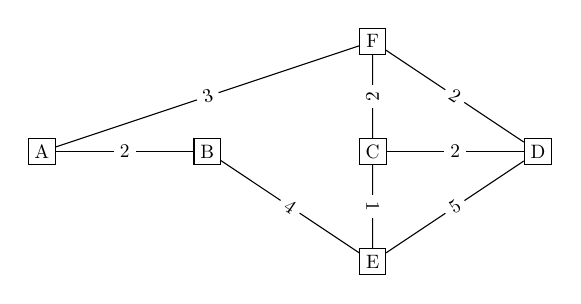
\begin{tikzpicture}[scale=0.7, transform shape]
            \node[draw] (A) at (0,0) {A};
            \node[draw] (B) at (3,0) {B};
            \node[draw] (C) at (6,0) {C};
            \node[draw] (D) at (9,0) {D};
            \node[draw] (E) at (6,-2) {E};
            \node[draw] (F) at (6,2) {F};
    
            \draw (A)--(B) node[sloped, midway, fill=white]{2};
            %\draw (B)--(C) node[sloped, midway, fill=white]{6};
            \draw (C)--(D) node[sloped, midway, fill=white]{2};
            \draw (A)--(F) node[sloped, midway, fill=white]{3};
            \draw (B)--(E) node[sloped, midway, fill=white]{4};
            \draw (F)--(C) node[sloped, midway, fill=white]{2};
            \draw (E)--(C) node[sloped, midway, fill=white]{1};
            \draw (E)--(D) node[sloped, midway, fill=white]{5};
            \draw (D)--(F) node[sloped, midway, fill=white]{2};
    
        \end{tikzpicture}
    \end{center}
    \begin{center}
        \begin{tabular}{|*{6}{c|}}
            \hline
            A & B      & C      & D      & E      & F      \\
            \hline
            0 & 2 (A) & 5 (F) & 7 (C) & 6 (B) & 3 (A) \\
            \hline
        \end{tabular}
    \end{center}
On remonte dans le tableau pour trouver le chemin vers une destination.\\
{\Large$$D \rightarrow C \rightarrow F \rightarrow A$$}
\end{frame}
\subsection{Complexité}
\begin{frame}[fragile]
    \frametitle{Complexité}
La complexité dépend de:
    \begin{itemize}
        \item<1-> du nombre de sommets (notée S): on visite chaque sommet
        \begin{lstlisting}[language=bash,basicstyle=\small,xleftmargin=0em, xrightmargin=0em]
Tant que (le nombre d'itérations) < (nombre de routeurs)
\end{lstlisting}
        \note{ligne 4 = on peut faire une amélioration: si pas de modification pendant l'itération, on peut s'arrêter }
        \item<2-> du nombre d'arcs (notée A): pour chaque sommet on regarde tous les arcs du graphe
        \begin{lstlisting}[language=bash,basicstyle=\small,xleftmargin=0em, xrightmargin=0em]
Pour chaque arc du graphe
\end{lstlisting}
    \end{itemize}

\end{frame}
\begin{frame}
    \frametitle{Complexité de l'algorithme de Bellman Ford}

    {\LARGE$$O(S.A)$$}
\note{précisément chaque arc est parcouru deux fois car on est dans un graphe non orienté}
\end{frame}

\section{OSPF: algorithme de Dijkstra}
\subsection{Principe}
\begin{frame}
    \frametitle{OSPF: algorithme de Dijkstra - principe}

    \begin{itemize}
        \item Edsger Dijkstra: mathématicien néerlandais
        \item Algorithme utilisé dans GPS
    \end{itemize}
    

    \note[item]{peut se contenter de renvoyer la distance départ/arrivée (et le chemin)}
    \note[item]{graphe non orienté possible}
    \note[item]{parfois appelé Moore-Dijkstra}
\end{frame}
\begin{frame}
    \frametitle{}

    \begin{aretenir}[]
        \underline{principe:} construire un sous-graphe en ajoutant à chaque itération un sommet de distance minimale.
    \end{aretenir}

\end{frame}
\begin{frame}
    \frametitle{}

    \begin{center}
        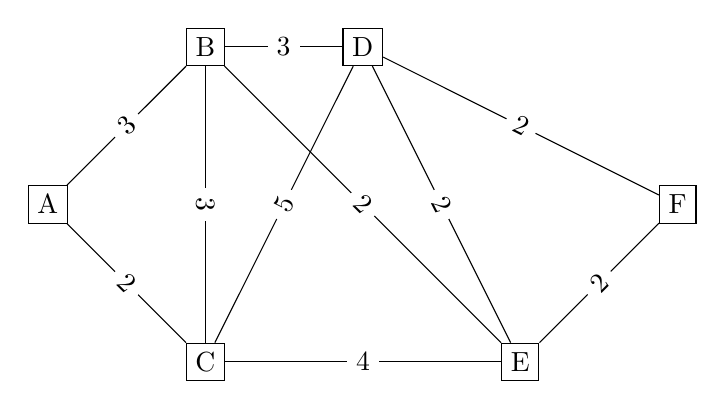
\begin{tikzpicture}
            \node[draw] (A) at (0,0) {A};
            \node[draw] (B) at (2,2) {B};
            \node[draw] (C) at (2,-2) {C};
            \node[draw] (D) at (4,2) {D};
            \node[draw] (E) at (6,-2) {E};
            \node[draw] (F) at (8,0) {F};
    
            \draw (A)--(B) node[sloped, midway, fill=white]{3};
            \draw (B)--(C) node[sloped, midway, fill=white]{3};
            \draw (A)--(C) node[sloped, midway, fill=white]{2};
            \draw (B)--(D) node[sloped, midway, fill=white]{3};
            \draw (B)--(E) node[sloped, midway, fill=white]{2};
            \draw (C)--(D) node[sloped, midway, fill=white]{5};
            \draw (C)--(E) node[sloped, midway, fill=white]{4};
            \draw (E)--(D) node[sloped, midway, fill=white]{2};
            \draw (D)--(F) node[sloped, midway, fill=white]{2};
            \draw (E)--(F) node[sloped, midway, fill=white]{2};
    
        \end{tikzpicture}
        \captionof{figure}{graphe non orienté et pondéré}
        \label{ospf}
    \end{center}

    \note{\begin{aretenir}[Remarque]
        Les poids de chaque arc représentent le coût de chaque connexion.
    \end{aretenir}
    coût 5 $\rightarrow$ 20Mbit/s\\
    coût 2 $\rightarrow$ 50Mbit/s}
\end{frame}


\subsection{Mise en application}
\begin{frame}[fragile]
    \frametitle{Mise en application}
\textbf{Initialisation:}
\begin{itemize}
    \item Créer un tableau des distances entre A et les routeurs, initialisées à l'infini.
    \item Modifier la distance vers A à 0.
\end{itemize}
\note[item]{S = suivant; V = voisin}
\note[item]{ligne 7: on compare encore la distance déjà enregistrée à distance du voisin + arc}
\end{frame}
\begin{frame}[fragile]
\textbf{Initialisation:}
\begin{itemize}
    \item Créer un tableau des distances entre A et les routeurs, initialisées à l'infini.
    \item Modifier la distance vers A à 0.
\end{itemize}
\textbf{Déroulement:}
\begin{itemize}
    \item Tant qu'il reste des routeurs non sélectionnés
    \begin{itemize}
        \item Parmi les routeurs non-sélectionnés, choisir celui (noté S) ayant la plus petite distance.
        \item Pour chaque routeur adjacent à S (noté V) et non déjà sélectionné:
            \begin{itemize}
                \item Si (la distance de V) > (la distance de S + poids S-V)
                \\\hspace{1cm}$\Rightarrow$ Mettre à jour la distance de V.
            \end{itemize}
    \end{itemize}
\end{itemize}
\note[item]{S = suivant; V = voisin}
\note[item]{ligne 7: on compare encore la distance déjà enregistrée à distance du voisin + arc}
\end{frame}

\begin{frame}
    \frametitle{Initialisation}

    \begin{center}
        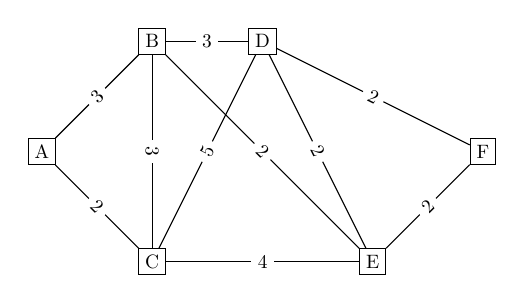
\begin{tikzpicture}[scale=0.7, transform shape]
            \node[draw] (A) at (0,0) {A};
            \node[draw] (B) at (2,2) {B};
            \node[draw] (C) at (2,-2) {C};
            \node[draw] (D) at (4,2) {D};
            \node[draw] (E) at (6,-2) {E};
            \node[draw] (F) at (8,0) {F};
    
            \draw (A)--(B) node[sloped, midway, fill=white]{3};
            \draw (B)--(C) node[sloped, midway, fill=white]{3};
            \draw (A)--(C) node[sloped, midway, fill=white]{2};
            \draw (B)--(D) node[sloped, midway, fill=white]{3};
            \draw (B)--(E) node[sloped, midway, fill=white]{2};
            \draw (C)--(D) node[sloped, midway, fill=white]{5};
            \draw (C)--(E) node[sloped, midway, fill=white]{4};
            \draw (E)--(D) node[sloped, midway, fill=white]{2};
            \draw (D)--(F) node[sloped, midway, fill=white]{2};
            \draw (E)--(F) node[sloped, midway, fill=white]{2};
    
        \end{tikzpicture}
    \end{center}
    \begin{center}
        \begin{tabular}{|*{6}{c|}}
            \hline
            A & B      & C      & D      & E      & F      \\
            \hline
            0 & \infty & \infty & \infty & \infty & \infty \\
            \hline
        \end{tabular}
    \end{center}

\end{frame}

\begin{frame}
    \frametitle{Sélection de A}

    \begin{center}
        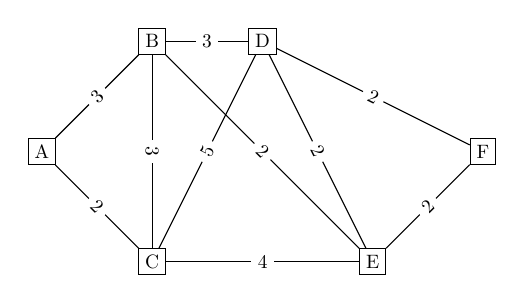
\begin{tikzpicture}[scale=0.7, transform shape]
            \node[draw] (A) at (0,0) {A};
            \node[draw] (B) at (2,2) {B};
            \node[draw] (C) at (2,-2) {C};
            \node[draw] (D) at (4,2) {D};
            \node[draw] (E) at (6,-2) {E};
            \node[draw] (F) at (8,0) {F};
    
            \draw (A)--(B) node[sloped, midway, fill=white]{3};
            \draw (B)--(C) node[sloped, midway, fill=white]{3};
            \draw (A)--(C) node[sloped, midway, fill=white]{2};
            \draw (B)--(D) node[sloped, midway, fill=white]{3};
            \draw (B)--(E) node[sloped, midway, fill=white]{2};
            \draw (C)--(D) node[sloped, midway, fill=white]{5};
            \draw (C)--(E) node[sloped, midway, fill=white]{4};
            \draw (E)--(D) node[sloped, midway, fill=white]{2};
            \draw (D)--(F) node[sloped, midway, fill=white]{2};
            \draw (E)--(F) node[sloped, midway, fill=white]{2};
    
        \end{tikzpicture}
    \end{center}
    \begin{center}
        \begin{tabular}{|*{6}{c|}}
            \hline
            A & B & C & D      & E      & F      \\
            \hline
            0 & \textbf{3 (A)} & \textbf{2 (A)} & \infty & \infty & \infty \\
            \hline
        \end{tabular}
        \hspace{2cm}
        \begin{tabular}{|c|}
            \hline
            nœuds visités \\
            \hline
            A             \\
            \hline
        \end{tabular}
    \end{center}

\end{frame}


\begin{frame}

    \begin{center}
        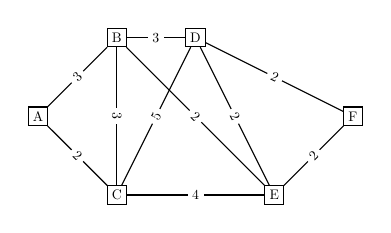
\begin{tikzpicture}[scale=0.5, transform shape]
            \node[draw] (A) at (0,0) {A};
            \node[draw] (B) at (2,2) {B};
            \node[draw] (C) at (2,-2) {C};
            \node[draw] (D) at (4,2) {D};
            \node[draw] (E) at (6,-2) {E};
            \node[draw] (F) at (8,0) {F};
    
            \draw (A)--(B) node[sloped, midway, fill=white]{3};
            \draw (B)--(C) node[sloped, midway, fill=white]{3};
            \draw (A)--(C) node[sloped, midway, fill=white]{2};
            \draw (B)--(D) node[sloped, midway, fill=white]{3};
            \draw (B)--(E) node[sloped, midway, fill=white]{2};
            \draw (C)--(D) node[sloped, midway, fill=white]{5};
            \draw (C)--(E) node[sloped, midway, fill=white]{4};
            \draw (E)--(D) node[sloped, midway, fill=white]{2};
            \draw (D)--(F) node[sloped, midway, fill=white]{2};
            \draw (E)--(F) node[sloped, midway, fill=white]{2};
    
        \end{tikzpicture}
    \end{center}
    On sélectionne le nœud non encore visité et avec la plus petite distance: C.
    \begin{center}
        \begin{tabular}{|*{6}{c|}}
            \hline
            A & B & C & D      & E      & F      \\
            \hline
            0 & 3 (A) & 2 (A) & \infty & \infty & \infty \\
            \hline
            \cellcolor{gray} & 3 (A) & 2 (A) & \textbf{7 (C)} & \textbf{6 (C)} & \infty \\
            \hline
        \end{tabular}
        \hspace{2cm}
        \begin{tabular}{|c|}
            \hline
            nœuds visités \\
            \hline
            A - C            \\
            \hline
        \end{tabular}
    \end{center}

\end{frame}
\begin{frame}
    \frametitle{}

    \begin{aretenir}[Observation]
        La route la plus courte a déjà été déterminée pour les nœuds déjà visités. Ils ne seront plus modifiés (cellule grise).
    \end{aretenir}

\end{frame}
\begin{frame}
    \frametitle{}

    \begin{activite}
        Continuer de dérouler l'algorithme sur le graphe.
        \end{activite}
        \begin{center}
            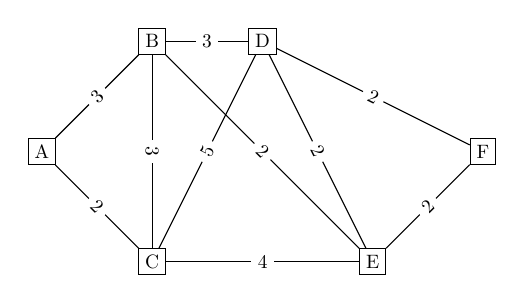
\begin{tikzpicture}[scale=0.7, transform shape]
                \node[draw] (A) at (0,0) {A};
                \node[draw] (B) at (2,2) {B};
                \node[draw] (C) at (2,-2) {C};
                \node[draw] (D) at (4,2) {D};
                \node[draw] (E) at (6,-2) {E};
                \node[draw] (F) at (8,0) {F};
        
                \draw (A)--(B) node[sloped, midway, fill=white]{3};
                \draw (B)--(C) node[sloped, midway, fill=white]{3};
                \draw (A)--(C) node[sloped, midway, fill=white]{2};
                \draw (B)--(D) node[sloped, midway, fill=white]{3};
                \draw (B)--(E) node[sloped, midway, fill=white]{2};
                \draw (C)--(D) node[sloped, midway, fill=white]{5};
                \draw (C)--(E) node[sloped, midway, fill=white]{4};
                \draw (E)--(D) node[sloped, midway, fill=white]{2};
                \draw (D)--(F) node[sloped, midway, fill=white]{2};
                \draw (E)--(F) node[sloped, midway, fill=white]{2};
        
            \end{tikzpicture}
        \end{center}
\end{frame}
\begin{frame}
    \frametitle{Correction}

    \begin{center}
        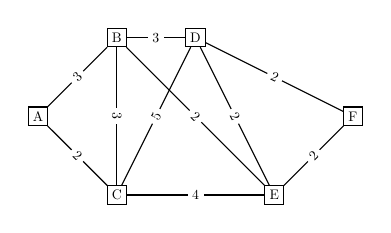
\begin{tikzpicture}[scale=0.5, transform shape]
            \node[draw] (A) at (0,0) {A};
            \node[draw] (B) at (2,2) {B};
            \node[draw] (C) at (2,-2) {C};
            \node[draw] (D) at (4,2) {D};
            \node[draw] (E) at (6,-2) {E};
            \node[draw] (F) at (8,0) {F};
    
            \draw (A)--(B) node[sloped, midway, fill=white]{3};
            \draw (B)--(C) node[sloped, midway, fill=white]{3};
            \draw (A)--(C) node[sloped, midway, fill=white]{2};
            \draw (B)--(D) node[sloped, midway, fill=white]{3};
            \draw (B)--(E) node[sloped, midway, fill=white]{2};
            \draw (C)--(D) node[sloped, midway, fill=white]{5};
            \draw (C)--(E) node[sloped, midway, fill=white]{4};
            \draw (E)--(D) node[sloped, midway, fill=white]{2};
            \draw (D)--(F) node[sloped, midway, fill=white]{2};
            \draw (E)--(F) node[sloped, midway, fill=white]{2};
    
        \end{tikzpicture}
    \end{center}
    On sélectionne le nœud non encore visité et avec la plus petite distance: B.
    \begin{center}
        \begin{tabular}{|*{6}{c|}}
            \hline
            A & B & C & D      & E      & F      \\
            \hline
            0 & 3 (A) & 2 (A) & \infty & \infty & \infty \\
            \hline
            \cellcolor{gray} & 3 (A) & 2 (A) & 7 (C) & 6 (C) & \infty \\
            \hline
            \cellcolor{gray} & 3 (A) & \cellcolor{gray} & \textbf{6 (B)} & \textbf{5 (B)} & \infty \\
            \hline
        \end{tabular}
        \hspace{2cm}
        \begin{tabular}{|c|}
            \hline
            nœuds visités \\
            \hline
            A - C - B           \\
            \hline
        \end{tabular}
    \end{center}
\note{C n'est pas regardé: on a déjà trouvé la + petite distance pour lui = il a déjà été visité}
\end{frame}

\begin{frame}
    \frametitle{Correction}

    \begin{center}
        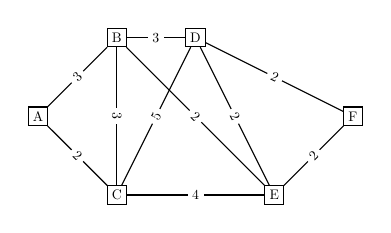
\begin{tikzpicture}[scale=0.5, transform shape]
            \node[draw] (A) at (0,0) {A};
            \node[draw] (B) at (2,2) {B};
            \node[draw] (C) at (2,-2) {C};
            \node[draw] (D) at (4,2) {D};
            \node[draw] (E) at (6,-2) {E};
            \node[draw] (F) at (8,0) {F};
    
            \draw (A)--(B) node[sloped, midway, fill=white]{3};
            \draw (B)--(C) node[sloped, midway, fill=white]{3};
            \draw (A)--(C) node[sloped, midway, fill=white]{2};
            \draw (B)--(D) node[sloped, midway, fill=white]{3};
            \draw (B)--(E) node[sloped, midway, fill=white]{2};
            \draw (C)--(D) node[sloped, midway, fill=white]{5};
            \draw (C)--(E) node[sloped, midway, fill=white]{4};
            \draw (E)--(D) node[sloped, midway, fill=white]{2};
            \draw (D)--(F) node[sloped, midway, fill=white]{2};
            \draw (E)--(F) node[sloped, midway, fill=white]{2};
    
        \end{tikzpicture}
    \end{center}
    On sélectionne le nœud non encore visité et avec la plus petite distance: E.
    \begin{center}
        \begin{tabular}{|*{6}{c|}}
            \hline
            A & B & C & D      & E      & F      \\
            \hline
            0 & 3 (A) & 2 (A) & \infty & \infty & \infty \\
            \hline
            \cellcolor{gray} & 3 (A) & 2 (A) & 7 (C) & 6 (C) & \infty \\
            \hline
            \cellcolor{gray} & 3 (A) & \cellcolor{gray} & 6 (B) & 5 (B) & \infty \\
            \hline
            \cellcolor{gray} & \cellcolor{gray} & \cellcolor{gray} & 6 (B) & 5 (B) & \textbf{7 (E)} \\
            \hline
        \end{tabular}
        \hspace{2cm}
        \begin{tabular}{|c|}
            \hline
            nœuds visités \\
            \hline
            A - C - B - E    \\
            \hline
        \end{tabular}
    \end{center}

\end{frame}

\begin{frame}
    \frametitle{Correction}

    \begin{center}
        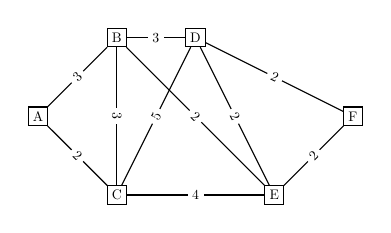
\begin{tikzpicture}[scale=0.5, transform shape]
            \node[draw] (A) at (0,0) {A};
            \node[draw] (B) at (2,2) {B};
            \node[draw] (C) at (2,-2) {C};
            \node[draw] (D) at (4,2) {D};
            \node[draw] (E) at (6,-2) {E};
            \node[draw] (F) at (8,0) {F};
    
            \draw (A)--(B) node[sloped, midway, fill=white]{3};
            \draw (B)--(C) node[sloped, midway, fill=white]{3};
            \draw (A)--(C) node[sloped, midway, fill=white]{2};
            \draw (B)--(D) node[sloped, midway, fill=white]{3};
            \draw (B)--(E) node[sloped, midway, fill=white]{2};
            \draw (C)--(D) node[sloped, midway, fill=white]{5};
            \draw (C)--(E) node[sloped, midway, fill=white]{4};
            \draw (E)--(D) node[sloped, midway, fill=white]{2};
            \draw (D)--(F) node[sloped, midway, fill=white]{2};
            \draw (E)--(F) node[sloped, midway, fill=white]{2};
    
        \end{tikzpicture}
    \end{center}
    On sélectionne le nœud non encore visité et avec la plus petite distance: D.
    \begin{center}
        \begin{tabular}{|*{6}{c|}}
            \hline
            A & B & C & D      & E      & F      \\
            \hline
            0 & 3 (A) & 2 (A) & \infty & \infty & \infty \\
            \hline
            \cellcolor{gray} & 3 (A) & 2 (A) & 7 (C) & 6 (C) & \infty \\
            \hline
            \cellcolor{gray} & 3 (A) & \cellcolor{gray} & 6 (B) & 5 (B) & \infty \\
            \hline
            \cellcolor{gray} & \cellcolor{gray} & \cellcolor{gray} & 6 (B) & 5 (B) & 7 (E) \\
            \hline
            \cellcolor{gray} & \cellcolor{gray} & \cellcolor{gray} & 6 (B) & \cellcolor{gray} & 7 (E) \\
            \hline
        \end{tabular}
        \hspace{2cm}
        \begin{tabular}{|c|}
            \hline
            nœuds visités \\
            \hline
            A - C - B - E - D   \\
            \hline
        \end{tabular}
    \end{center}
\note{pas de modification}
\end{frame}

\begin{frame}
    \frametitle{Correction}

    \begin{center}
        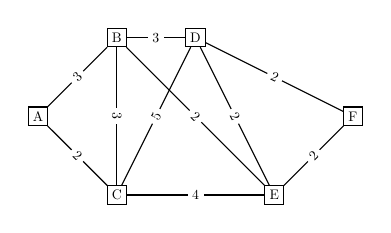
\begin{tikzpicture}[scale=0.5, transform shape]
            \node[draw] (A) at (0,0) {A};
            \node[draw] (B) at (2,2) {B};
            \node[draw] (C) at (2,-2) {C};
            \node[draw] (D) at (4,2) {D};
            \node[draw] (E) at (6,-2) {E};
            \node[draw] (F) at (8,0) {F};
    
            \draw (A)--(B) node[sloped, midway, fill=white]{3};
            \draw (B)--(C) node[sloped, midway, fill=white]{3};
            \draw (A)--(C) node[sloped, midway, fill=white]{2};
            \draw (B)--(D) node[sloped, midway, fill=white]{3};
            \draw (B)--(E) node[sloped, midway, fill=white]{2};
            \draw (C)--(D) node[sloped, midway, fill=white]{5};
            \draw (C)--(E) node[sloped, midway, fill=white]{4};
            \draw (E)--(D) node[sloped, midway, fill=white]{2};
            \draw (D)--(F) node[sloped, midway, fill=white]{2};
            \draw (E)--(F) node[sloped, midway, fill=white]{2};
    
        \end{tikzpicture}
    \end{center}
    On sélectionne le nœud non encore visité et avec la plus petite distance: F.
    \begin{center}
        \begin{tabular}{|*{6}{c|}}
            \hline
            A & B & C & D      & E      & F      \\
            \hline
            0 & 3 (A) & 2 (A) & \infty & \infty & \infty \\
            \hline
            \cellcolor{gray} & 3 (A) & 2 (A) & 7 (C) & 6 (C) & \infty \\
            \hline
            \cellcolor{gray} & 3 (A) & \cellcolor{gray} & 6 (B) & 5 (B) & \infty \\
            \hline
            \cellcolor{gray} & \cellcolor{gray} & \cellcolor{gray} & 6 (B) & 5 (B) & 7 (E) \\
            \hline
            \cellcolor{gray} & \cellcolor{gray} & \cellcolor{gray} & 6 (B) & \cellcolor{gray} & 7 (E) \\
            \hline
            \cellcolor{gray} & \cellcolor{gray} & \cellcolor{gray} & \cellcolor{gray} & \cellcolor{gray} & 7 (E)\\
            \hline
        \end{tabular}
        \hspace{2cm}
        \begin{tabular}{|c|}
            \hline
            nœuds visités \\
            \hline
            A - C - B - E - D - F  \\
            \hline
        \end{tabular}
    \end{center}
\note{pas de modification}
\end{frame}

\begin{frame}
    \frametitle{Correction}

    \begin{center}
        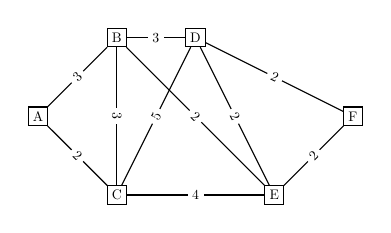
\begin{tikzpicture}[scale=0.5, transform shape]
            \node[draw] (A) at (0,0) {A};
            \node[draw] (B) at (2,2) {B};
            \node[draw] (C) at (2,-2) {C};
            \node[draw] (D) at (4,2) {D};
            \node[draw] (E) at (6,-2) {E};
            \node[draw] (F) at (8,0) {F};
    
            \draw (A)--(B) node[sloped, midway, fill=white]{3};
            \draw (B)--(C) node[sloped, midway, fill=white]{3};
            \draw (A)--(C) node[sloped, midway, fill=white]{2};
            \draw (B)--(D) node[sloped, midway, fill=white]{3};
            \draw (B)--(E) node[sloped, midway, fill=white]{2};
            \draw (C)--(D) node[sloped, midway, fill=white]{5};
            \draw (C)--(E) node[sloped, midway, fill=white]{4};
            \draw (E)--(D) node[sloped, midway, fill=white]{2};
            \draw (D)--(F) node[sloped, midway, fill=white]{2};
            \draw (E)--(F) node[sloped, midway, fill=white]{2};
    
        \end{tikzpicture}
    \end{center}
    On sélectionne le nœud non encore visité et avec la plus petite distance: F.
    \begin{center}
        \begin{tabular}{|*{6}{c|}}
            \hline
            A & B & C & D      & E      & F      \\
            \hline
            0 & 3 (A) & 2 (A) & \infty & \infty & \infty \\
            \hline
            \cellcolor{gray} & 3 (A) & 2 (A) & 7 (C) & 6 (C) & \infty \\
            \hline
            \cellcolor{gray} & 3 (A) & \cellcolor{gray} & 6 (B) & 5 (B) & \infty \\
            \hline
            \cellcolor{gray} & \cellcolor{gray} & \cellcolor{gray} & 6 (B) & 5 (B) & 7 (E) \\
            \hline
            \cellcolor{gray} & \cellcolor{gray} & \cellcolor{gray} & 6 (B) & \cellcolor{gray} & 7 (E) \\
            \hline
            \cellcolor{gray} & \cellcolor{gray} & \cellcolor{gray} & \cellcolor{gray} & \cellcolor{gray} & 7 (E) \\
            \hline
            \cellcolor{gray} & \cellcolor{gray} & \cellcolor{gray} & \cellcolor{gray} & \cellcolor{gray} & \cellcolor{gray} \\
            \hline
        \end{tabular}
        \hspace{2cm}
        \begin{tabular}{|c|}
            \hline
            nœuds visités \\
            \hline
            A - C - B - E - D - F  \\
            \hline
        \end{tabular}
    \end{center}
\note{tous les nœuds ont été visités = fin de l'algorithme. On peut reconstruire le chemin.\\
pour F: F $\rightarrow$ E $\rightarrow$ B $\rightarrow$ A}
\end{frame}
\begin{frame}
    \frametitle{}
    \begin{center}
        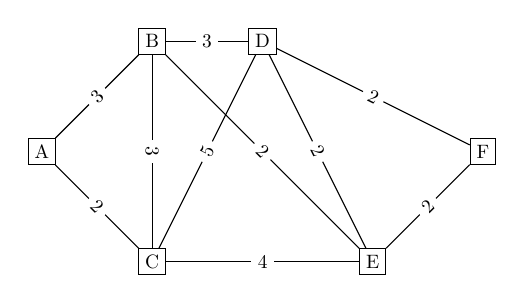
\begin{tikzpicture}[scale=0.7, transform shape]
            \node[draw] (A) at (0,0) {A};
            \node[draw] (B) at (2,2) {B};
            \node[draw] (C) at (2,-2) {C};
            \node[draw] (D) at (4,2) {D};
            \node[draw] (E) at (6,-2) {E};
            \node[draw] (F) at (8,0) {F};
    
            \draw (A)--(B) node[sloped, midway, fill=white]{3};
            \draw (B)--(C) node[sloped, midway, fill=white]{3};
            \draw (A)--(C) node[sloped, midway, fill=white]{2};
            \draw (B)--(D) node[sloped, midway, fill=white]{3};
            \draw (B)--(E) node[sloped, midway, fill=white]{2};
            \draw (C)--(D) node[sloped, midway, fill=white]{5};
            \draw (C)--(E) node[sloped, midway, fill=white]{4};
            \draw (E)--(D) node[sloped, midway, fill=white]{2};
            \draw (D)--(F) node[sloped, midway, fill=white]{2};
            \draw (E)--(F) node[sloped, midway, fill=white]{2};
    
        \end{tikzpicture}
    \end{center}
    \begin{center}
        \begin{tabular}{|*{6}{c|}}
            \hline
            A & B & C & D      & E      & F      \\
            \hline
            0 & 3 (A) & 2 (A) & 6 (B) & 5 (B) & 7 (E) \\
            \hline
        \end{tabular}
    \end{center}
    On remonte dans le tableau pour trouver le chemin vers une destination.\\
{\Large$$F \rightarrow E \rightarrow B \rightarrow A$$}
\end{frame}


\subsection{Complexité}
\begin{frame}[fragile]
    \frametitle{Complexité}

    \begin{itemize}
        \item<1->La complexité dépend du nombre de sommets S et du nombre d'arcs A.
        \item<2->Le point clé de l'algorithme tient dans la recherche de la distance minimale.
        \begin{center}
        \begin{lstlisting}[language=bash, basicstyle=\small, xleftmargin=1.5em, xrightmargin=1.5em]
Parmi les routeurs non-sélectionnés, choisir le routeur (noté S) ayant la plus petite distance.        
\end{lstlisting}
        \end{center}
    \end{itemize}
\note[item]{hors programme}
\note[item]{utilisation de tas par exemple}
\end{frame}

\begin{frame}
    \frametitle{Complexité de l'algorithme de Dijkstra}

    {\LARGE $$O((A+S)×\log{S})$$    }

\end{frame}
\end{document}
